%!TEX TS-program = xelatex
%!TEX encoding = UTF-8 Unicode

\documentclass{article}



\usepackage{graphicx}      % needed to embed pictures (e.g., pdf, jpg, png)

\usepackage{fontspec}      % needed to specify document fonts
\usepackage{unicode-math}  % needed to use unicode math fonts

\setmainfont{STIX Two Text}                % specify default font
\setmathfont{STIX Two Math}                % specify default math font
% STIX fonts are available at https://www.stixfonts.org

\usepackage[backend=biber,
            maxbibnames=99,
            style=authoryear-icomp]{biblatex} % used for bibliographic references

\addbibresource{myrefs.bib} % the file where you store bibliographic information



\begin{document}
% everything beyond this point will show up in your actual document

\begin{center} % the title
	\LARGE\bfseries
	A Minimal Modern \LaTeX{} Document
\end{center}

\vspace{3ex} % a bit of vertical space

Note that you can go crazy with unicode accents and glyphs (e.g., àñëîøξåǔōę), without using backslash even once!

\section{A short section with an equation}

Lorem ipsum dolor sit amet, consectetur adipiscing elit. Curabitur pretium eros eu urna vehicula ultricies. In at tempus lorem. Suspendisse viverra metus et ex tristique cursus. Vivamus vel diam ullamcorper ipsum semper tincidunt.

\begin{equation} % a numbered math equation
	E = mc^2
	\label{eq:energy} % use this label for referencing this particular equation
\end{equation}

\subsection{Examples of in-text references}
\label{sec:refs}

We are currently within section~\ref{sec:refs}, on page \pageref{sec:refs} of the document.
Here is a reference to equation~(\ref{eq:energy}).
Here is a reference to figure~\ref{fig:avar}.
And here is a bibliographic reference in \textit{author-year} style \parencite{Pesnin_2024}.

%\clearpage % start a new page before processing subsequent floats (e.g., figures)

\begin{figure}[b!] % a figure with a numbered caption
	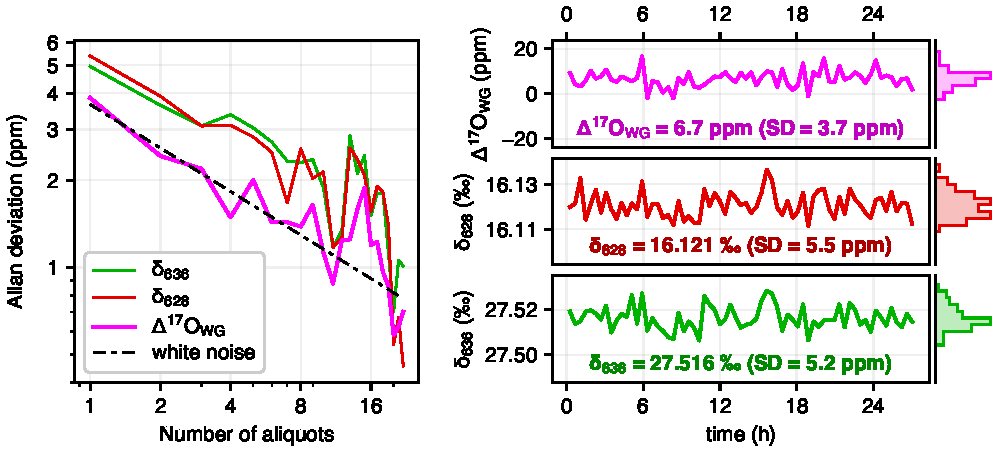
\includegraphics[width=\textwidth]{avar}
	\caption{Colorful data}
	\label{fig:avar} % use this label for referencing this particular figure
\end{figure}

\printbibliography % the list of references

\end{document}